
\documentclass[../summary.tex]{subfiles}

\begin{document}
	
	\section{Energie rechtvaardigheid}
	\subsection{Energie transitie}
	
	De \textbf{energietransitie} heeft enerzijds een hele hoop \textbf{technische uitdagingen}. We moeten er bijvoorbeeld voor zorgen dat we elektrolyse kunnen doen op een manier die genoeg energie-efficiënt is. We hebben nucleair afval dat we ergens moeten opslaan. We maken gebruik van zonnepanelen, maar de zon schijnt niet altijd, dus we moeten het elektriciteitsnet balanceren aangezien de stroomproductie zeer variabel is. Dit zijn allemaal hele lastige technologische uitdagingen. \\
	\\
	Aan de andere kant zijn er ook \textbf{sociale uitdagingen} van de energietransitie. Een voorbeeld hiervan zijn de extreem hoge energieprijzen. In het geval van armoede, energiearmoede bijvoorbeeld. Energie-infrastructuur moet ook ergens staan en mensen hebben dat het liefst niet in hun buurt. Hierdoor ontstaan er protesten die dan meestal gaan over het feit dat mensen erop tegen zijn dat de energie-infrastructuur door hun achtertuin moet lopen. We hebben daarnaast ook allerlei materialen nodig voor het maken van windmolens, zonnepanelen enzovoort. Die materialen komen heel vaak van plaatsen en gemeenschappen waar arbeidsomstandigheden zeer slecht zijn. Tenslotte hebben we heel veel infrastructuur nodig die soms door natuurreservaten lopen om de energie bij de gebruikers te krijgen, maar dit is voor de natuur en de mensen daar niet geweldig. Dit soort problemen zijn minstens zo groot als de technologische aspecten. 
	
	\subsection{Verdelen van het werk}
	
	Hoe moeten de technische en sociale uitdagingen verdeeld worden?  Er zijn drie mogelijke opvattingen mogelijk:

	\begin{description}
		\item[Separatisme] De technische zaken worden overgelaten aan ingenieurs, terwijl de niet-technische zaken worden opgelost door anderen zoals filosofen en politici.
		\item [Technocratie] Ingenieurs beslissen alles. Zij lossen zowel de technische en sociale challenges op.
		\item [Whistle-blowing] Ingenieurs richten zich op technische problemen, maar als hen gevraagd wordt om iets onethisch te doen, kunnen ze kiezen om aan de bel te trekken (whistle-blowing). De sociale problemen worden overgelaten aan de niet-ingenieurs.
	\end{description}
	
	\begin{figure}[H]
		\centering
		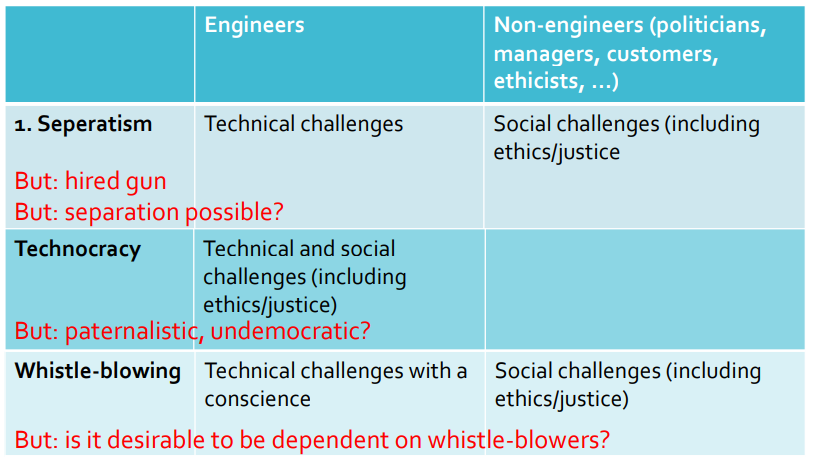
\includegraphics[width=0.8\linewidth]{../images/division-of-labour-table}
		\caption{Samenvattende tabel van de verschillende werkverdelingen}
		\label{fig:division-of-labour-table}
	\end{figure}
	\newpage
		
	\subsubsection{Problemen bij separatisme}
	Bij separatisme treden er \textbf{twee problemen} op.
	\begin{description}
		\item[Hired Gun] Iemand die betaald wordt om technologie te ontwikkelen zonder verantwoordelijkheid te nemen voor de ethische implicaties ervan. Dit probleem kan relevant  zijn voor toekomstige ingenieurs, die mogelijk geconfronteerd worden met de keuze om technologieën te ontwikkelen waar ze niet volledig achter staan.
	\end{description}
	Een voorbeeld hiervan is \textbf{Wernher von Braun}, hij was een hired gun, een ingenieur die tijdens het nazisme in Duitsland werkte en later naar de Verenigde Staten ging om technologische ontwikkelingen te bevorderen. "Once the rockets go up, who cares where they come down, that's not my department." is zijn bekendste quote.
	
	\begin{description}
		\item[Is separatisme mogelijk?] Dit kan uitgelegd worden door middel van volgend voorbeeld.
	\end{description}
	Enerzijds heb je \textbf{Joseph Pitt} die zegt: \textbf{`Guns don't kill people, people kill people'}. Hiermee beweerd hij dat technologische artefacten geen waarden hebben of bevatten. Technologie is neutraal. Wij bepalen hoe we ze gebruiken. Dit kan worden gelinkt aan de \textbf{`Value Neutrality Thesis (VNT)'} en laat zien dat \textbf{separatisme mogelijk} is.\\
	\\
	Aan de andere kant heb je \textbf{Langdon Winner} die zegt: \textbf{`Actually, Guns do kill people'}. Hij beweert dus dat \textbf{technologische artefacten} wel degelijk \textbf{politiek geladen} kunnen zijn. Hij illustreert dit met het voorbeeld van bruggen ontworpen door architect Robert Moses in New York, die met opzet te laag waren voor bussen, waardoor vooral autobezitters toegang kregen tot bepaalde gebieden. Winner benadrukt dat technologieën niet neutraal zijn en inherent waarden bevatten, zoals in dit geval een racistische geladen. Hierdoor is \textbf{separatie dus niet mogelijk}.\\
	\\
	\textbf{Pitt} vindt het idee van waarden in technologische objecten belachelijk. Hij \textbf{vraagt waar die waarden dan zouden zitten - in welke steen, in welke hoogte?} Hij betoogt dat technologie niet intrinsiek waarden bevat en dat mensen verantwoordelijkheid moeten nemen voor hun handelingen. Hij \textbf{verwerpt het idee dat technologieën onethisch gedrag veroorzaken}, en benadrukt dat het de mensen zijn die verantwoordelijk zijn voor hun acties.\\
	\\
	De nuance in deze kwestie wordt benadrukt door \textbf{Michael Klenk}. Klenk introduceert het concept van \textbf{`affordances'} en stelt dat ingenieurs intenties en waarden hebben die vaak het ontwerp van een artefact beïnvloeden. Dit bepaalt op zijn beurt vaak hoe het artefact wordt gebruikt, hoewel de relatie niet strikt deterministisch is. Klenk legt uit dat artefacten bepaalde handelingen waarschijnlijker maken dan andere, vergelijkbaar met hoe een knop de neiging heeft om mensen in de richting van indrukken te sturen.
	
	\begin{figure}[H]
		\centering
		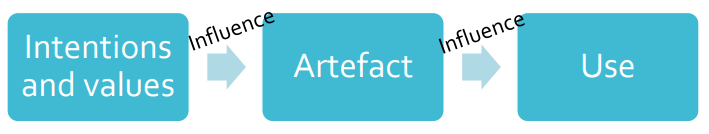
\includegraphics[width=0.7\linewidth]{../images/affordances}
		\caption{Hoe intenties en waardes het gebruik van een artefact beïnvloeden}
		\label{fig:affordances}
	\end{figure}
	
	\ \\
	Klenk's perspectief impliceert dat er \textbf{wel degelijk waarden in een artefact worden ingebracht door de ingenieur}, wat de vraag oproept over de verantwoordelijkheid van ingenieurs bij het creëren van technologieën. Als de intenties en waarden van de ingenieur op de een of andere manier in het artefact terechtkomen, suggereert dit dat het \textbf{niet volledig mogelijk} is \textbf{om sociale en technologische waarden te scheiden}. Dit werpt vragen op over de verantwoordelijkheid van degenen die technologieën ontwikkelen en of het idee van separatisme wel haalbaar is als waarden daadwerkelijk in de artefacten worden ingebed.
	
	\subsubsection{Probleem van technocratie}
	
	Ingenieurs begrijpen wellicht niet alle perspectieven. De technocratie kan als \textbf{paternalistisch} en \textbf{ondemocratisch} beschouwd worden, omdat \textbf{ingenieurs beperkt zijn tot hun eigen achtergrond en perspectief}. Dit beperkte standpunt kan leiden tot een gebrek aan representatie van diverse perspectieven. Daarnaast \textbf{zou het ondemocratisch zijn als één groep alle beslissingen neemt}. De technocratie wordt dus als niet de beste oplossing gezien.
	
	\subsubsection{Probleem van whistle-blowing}
	
	Dit model plaatst een \textbf{aanzienlijke druk op de ingenieurs}, aangezien de verantwoordelijkheid voor \textbf{ethische beslissingen volledig bij hen} ligt. Whistle-blowing kan leiden tot het openbaar maken van vertrouwelijke informatie en kan de carrière van de ingenieur in gevaar brengen. Het is niet ideaal om volledig te vertrouwen op de morele integriteit van individuele ingenieurs om ethische kwesties in de aan te pakken. Het kan inefficiënt zijn en kan problemen veroorzaken als niet alle ingenieurs dezelfde morele normen hanteren.
	
	\subsubsection{Conclusie}
	
	Alle drie de werkverdelingen, i.e. separatisme, technocratie en whistle-blowing, zijn niet ideaal.
	
	\subsection{Link tussen rechtvaardigheid en energie}
	
	De link werd heel expliciet gemaakt eigenlijk eind van de 20ste eeuw. In de late 20ste eeuw kwam in North Carolina een \textbf{Environmental Justice beweging} op gang \textbf{als reactie op het lozen van toxische stoffen in het watersysteem}. Deze beweging benadrukte dat de milieuproblemen niet eerlijk waren verdeeld en dat bepaalde gemeenschappen onevenredig werden getroffen.\\
	\\
	\textbf{Uit onderzoek bleek dat raciale factoren een aanzienlijke rol speelden in de locatie van gevaarlijke afvalfaciliteiten in de Verenigde Staten}. Met behulp van een kaart waarop de woonplaatsen van mensen met een bepaalde etnische achtergrond werden aangegeven, kon worden voorspeld waar de meest giftige stoffen werden geloosd. Dit leidde tot de term "environmental racism," waarbij de conclusie was dat minderheidsgroepen, met name \textbf{mensen met een kleur}, \textbf{onevenredig} werden \textbf{blootgesteld aan schadelijke gevolgen} van het energiesysteem.\\
	\\
	Een paar andere voorbeelden zijn de milieu-impact van \textbf{mijnbouwactiviteiten} voor de productie van benodigde materialen, de aardbevingen veroorzaakt door langdurige \textbf{gaswinning}, en de opkomende kwestie van \textbf{energiearmoede} als gevolg van stijgende energieprijzen.\\
	\\
	Dit brengt ons bij het volgende. \textbf{Wat is dan de link met rechtvaardigheid en energie?} Het komt er op neer \textbf{dat energiesystemen onrechtvaardigheden kunnen veroorzaken}. Het gebeurt niet altijd, maar het kan. Een van die onrechtvaardigheden heeft vooral te maken met rijkdom en de verdelingen van wie de voordelen en wie de lasten krijgt.
	
	\subsection{Utopie}
	
	\textbf{Ingenieurs maken technologieën}, zoals windmolens, \textbf{die de wereld beïnvloeden}. Wat belangrijk is, is dat wij allemaal een idee hebben over hoe de wereld eruit zou moeten. Wij willen allemaal een wereld die eerlijk is, die tof is, die groen is. En dat soort ideeën beïnvloeden dus gigantisch hoe onze wereld eruit ziet. Dus \textbf{beslissingen zijn vaak niet neutraal}. Die worden ingegeven door allerlei ideeën, door allerlei waarden. En een van die dingen is \textbf{utopie}. \\
	\\
	Een utopie is een soort van maatschappij, land, stad of eiland. Een \textbf{denkbeeldige samenleving die (bijna) perfect is}. Het geeft een beeld van hoe we eigenlijk samen graag met elkaar zouden willen leven. Een utopie is een \textbf{`no place'}. Het is er niet en het kan waarschijnlijk ook niet.\\
	\\
	Een utopie, of het beeld van een ideale toekomstige samenleving, heeft \textbf{aanzienlijke invloed op verschillende aspecten van de maatschappij}. Het kan bijvoorbeeld de financiering van projecten stimuleren, samenwerking tussen gelijkgestemde partners bevorderen, het publieke debat vormgeven en zelfs de politieke agenda beïnvloeden. Deze invloeden hebben op hun beurt gevolgen voor welke technologieën worden ontwikkeld en hoe deze worden gerealiseerd, vaak via financieringsmechanismen die gericht zijn op het verwezenlijken van de utopische visie. Kortom, utopieën hebben een aanzienlijke impact op de koers van technologische ontwikkelingen en maatschappelijke veranderingen.
	
	\begin{figure}[H]
		\centering
		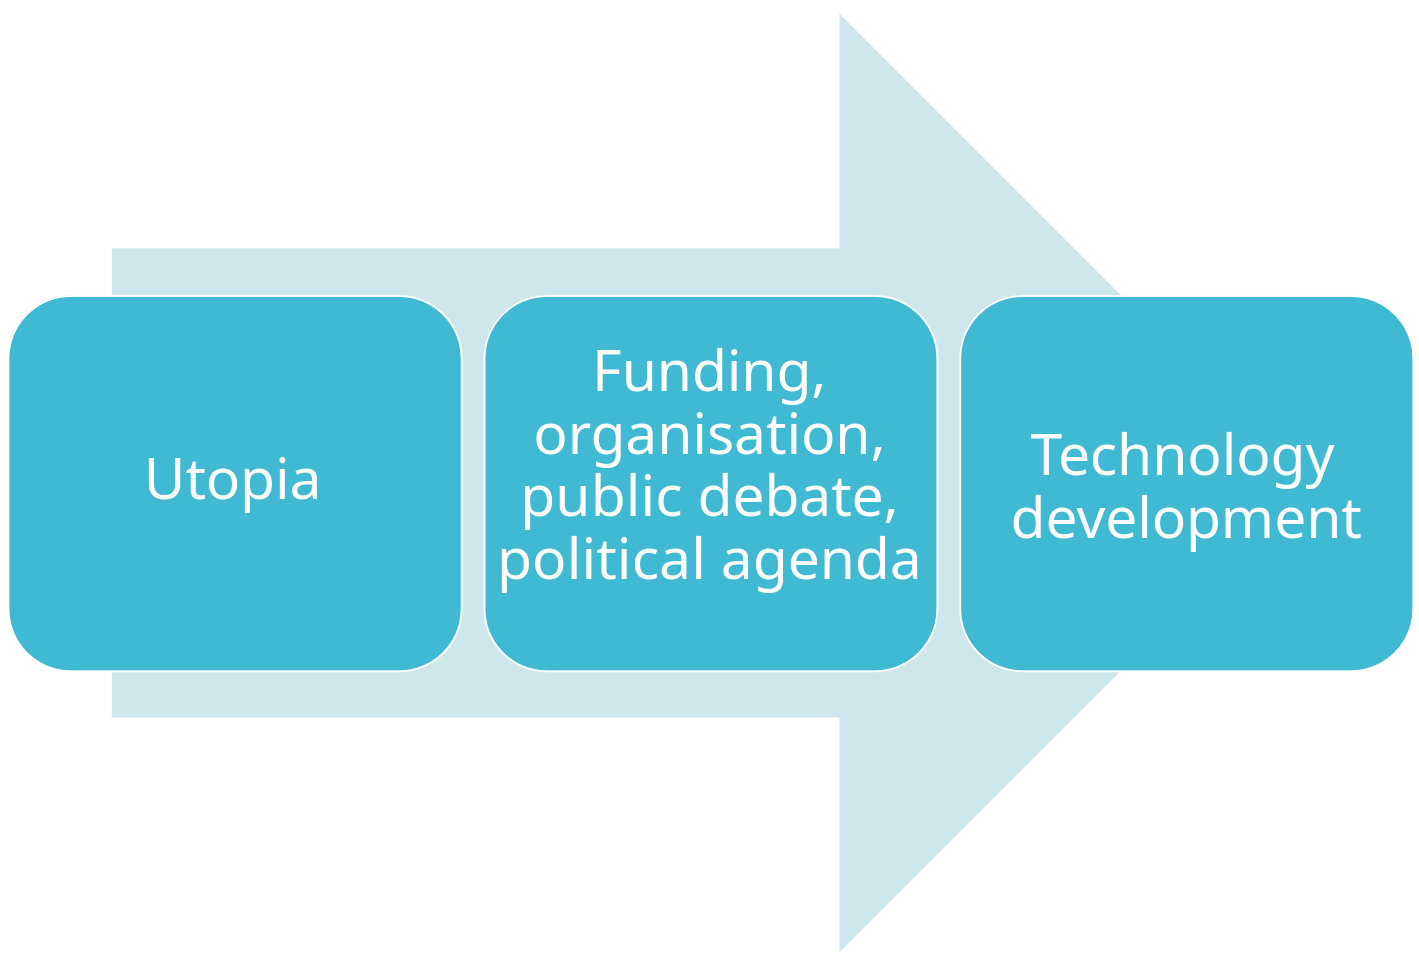
\includegraphics[width=0.7\linewidth]{../images/wat-utopieen-doen}
		\caption{Wat utopieën kunnen veroorzaken}
		\label{fig:wat-utopieen-doen}
	\end{figure}
	\ \\
	In het verleden zijn er verschillende energie-utopieën geweest die de visie op schone en oneindige energie benadrukten. In de vroege 20e eeuw werd kolenenergie gezien als een schone en onuitputtelijke bron. Later, in de jaren 1950, kwam nucleaire energie naar voren met de overtuiging dat het een overvloedige bron van schone energie zou zijn. Een andere opvallende utopie was gericht op waterstof, waarbij de gedachte was dat het kleinste element overal aanwezig was en dat decentralisatie van waterstofproductie macht en geld zou herverdelen. Dergelijke utopische ideeën hebben de ontwikkelingen op het gebied van energie sterk beïnvloed.\\
	\\
	Er zijn twee soorten energie-utopieën:
	\begin{description}
		\item[Abundance (overvloed)] Een eindeloze toevoer van energie; zorgen maken over de betaalbaarheid en toegang tot energie is niet langer nodig, omdat er voldoende energie is om al onze dromen waar te maken.
		\item [Sufficiency (voldoende)] Het bekritiseren van (kapitalistische) levensstijlen van welvaart en overvloed en het voorstellen van een minimalistische en ecologisch evenwichtige levensstijl waarin voldoende energie wordt geleverd om alleen die behoeften te vervullen die ons echt gelukkig maken.
	\end{description}
	\ \\
	Deze utopieën sturen technologische ontwikkeling en innovaties. Daarom is het heel belangrijk om daar kritisch over na te denken. Het voordeel van een energie-utopie zoals \textbf{`abundance'} is dat het mensen heel hard kan \textbf{motiveren om mee te doen aan de energietransitie}, maar \textbf{er zijn vier risico's}.
	\newpage
	\ \\
	Het  eerste risico is de \textbf{`dangerous illusion risk'}. Het streven naar een volledig circulaire economie en een wereld van overvloed is mogelijks onrealistisch, het is wellicht een illusie. Het geloof in een dergelijke overvloedige toekomst is gebaseerd op de hoop op technologische doorbraken of mirakeltechnologieën. Het gevaar van het nastreven van zo'n ideaalbeeld kan leiden tot het negeren van de werkelijke ecologische impact en kan leiden tot een snelle uitputting van materialen.\\
	\\
	Het tweede risico is de \textbf{`global justice risk'}.  Is overvloed wel verenigbaar met rechtvaardigheid? Het idee van overvloed voor bepaalde regio's kan leiden tot het negeren van de herkomst van materialen en mijnbouwpraktijken elders in de wereld, wat kan bijdragen aan onrechtvaardigheden.\\
	\\
	Het derde risico is de \textbf{`virtue ethics (deugdethiek): immoral risk'}. Je kan zeggen dat overvloed aan de ene kant en schaarste aan de andere kant beide ethische problemen zijn. Het maakt ons ongelukkig. Frugaliteit, ergens in het midden, kan gezien worden als een beter oplossing.
	
	\begin{figure}[H]
		\centering
		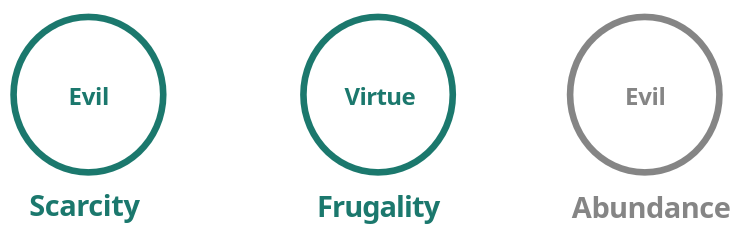
\includegraphics[width=0.6\linewidth]{../images/immorial-risk}
		\caption{Immorial risk}
		\label{fig:immorial-risk}
	\end{figure}
	
	\ \\
	Het laatste risico is de \textbf{`alienation (vervreemding) risk'}. Hiervoor kan verwezen worden naar het boek "The Dispossessed" van Ursula K. Le Guin. De boodschap van het boek is dat \textbf{overvloed} aan energie schadelijk kan zijn voor mensen, waardoor ze \textbf{ongelukkig} worden en \textbf{onstabiele sociale structuren} creëren, e.g. mensen die niks meer doen voor elkaar. Het kan ook leiden tot \textbf{vervreemding van de natuur}, waar mensen niet langer weten waar energie vandaan komt en losraken van de oorsprong van de bronnen.\\
	\\
	Hierdoor kunnen we onszelf afvragen of we moeten streven naar \textbf{abundance} of \textbf{sufficiency}. Misschien is sufficiency het beste, maar het blijft zeer complex. Als we zouden streven naar sufficiency krijgen we misschien de mensen niet mee. Hierdoor zal de energie-transitie niet lukken.\\
	\\
	Deze onzekerheid over wat het beste is om naar te streven, valt ook op als je kijkt naar verschillende klimaatbeleidsdocumenten. De EU \& USA Green Deal zijn sterk gericht op overvloed (abundance). Daarentegen bevatten de Paris Agreement en de Sustainable Development Goals (SDGs) veel minder tekstuele verwijzingen naar overvloed en neigen deze documenten eerder  naar het streven richting sufficiency wereldwijd.
	\newpage
	
	\subsection{Ontwerpen voor rechtvaardigheid}
	
	\subsubsection{Verschillende soorten van rechtvaardigheid}
	
	\begin{description}
		\item[Distributieve rechtvaardigheid] Draait om een rechtvaardige verdeling van lusten en lasten, waarbij goederen, risico's en andere elementen op een eerlijke manier worden verdeeld. 
		
		Hierbij worden volgende vragen gesteld met betrekking tot een energietechnologie of energiesysteem: Wat zijn de lasten (negatieve aspecten) en lusten (positieve aspecten)? Wie krijgt wat? En uiteindelijk, is deze verdeling eerlijk?
		
		Distributieve rechtvaardigheid is essentieel in het evalueren van de impact van energietechnologieën en systemen op de samenleving.
		
		\item[Procedurele rechtvaardigheid] Draait om de vraag hoe beslissingen worden genomen, wie erbij betrokken is, wie macht heeft en of het proces als geheel als eerlijk wordt beschouwd.
		
		In het geval van technologie worden deze vaak door ingenieurs en bedrijven gemaakt, met inspraak van aandeelhouders. Er is echter een groeiende roep voor meer inspraak van verschillende belanghebbenden tijdens het ontwerpproces, zodat het niet enkel beperkt is tot de aandeelhouders.
		
		In het geval van bijvoorbeeld een zonnepark naast een stad, welk niveau van de overheid (nationaal, regionaal, lokaal) moet de beslissing nemen en of mogen de bewoners van de stad inspraak hebben? Zo ja, welk niveau van inspraak hebben ze en kunnen ze alleen adviseren of zelfs een veto uitspreken?
		
		\item[Rechtvaardigheid tot erkenning] Heeft te maken heeft met de culturele kant van onrechtvaardigheid. 
		
		Wanneer mensen betrokken zijn bij energieprojecten, zoals de plaatsing van een zonnepark of windpark, klagen ze vaak dat ze zich niet erkend voelen. Erkenning houdt verband met de culturele en sociale normen die onrechtvaardig kunnen zijn. Naast de rechtvaardigheid van beslissingen en uitkomsten, kunnen sociale normen en culturele normen zelf ook onrechtvaardig zijn. 
		
		Bijvoorbeeld, als er discriminatie plaatsvindt op basis van huidskleur, beperkingen, gender, religie, dan wordt dat als onrechtvaardig beschouwd. Erkenning gaat over de devaluatie van bepaalde groepen, vooroordelen, en het structureel uitsluiten van bepaalde groepen. Mensen voelen zich vaak niet erkend als deze vormen van onrechtvaardigheid zich voordoen. Het idee is dat rechtvaardigheid niet alleen gaat over het verdelen van middelen, maar ook over sociale normen en de hiërarchie van waarden in de samenleving.
	\end{description}
		
	\subsubsection{Design for values}
	
	Het idee van \textbf{`design for values'} is om waarden in het ontwerp van technologieën op te nemen om ervoor te zorgen dat het uiteindelijke product bepaalde positieve handelingen mogelijk maakt. De `design for values'-benadering omvat drie fasen:
	
	\begin{description}
		\item[Discovery Phase] In deze fase denken ontwerpers na over welke waarden belangrijk zijn voor het ontwerp. Rechtvaardigheid is een voorbeeld van zo'n waarde, maar er zijn ook andere mogelijke waarden, zoals veiligheid, efficiëntie en kosteneffectiviteit.
		
		\item[Translation Phase] Na het identificeren van de waarden in de discovery phase, moeten deze waarden in het ontwerp worden geïntegreerd. Bijvoorbeeld, als veiligheid een waarde is, moet worden bepaald wat dat betekent in de context van het ontwerp. Dit kan specifieker worden gemaakt door operationele criteria te definiëren, zoals flammability (ontvlambaarheid). Deze operationele criteria kunnen vervolgens gemeten worden aan de hand van bepaalde standaarden en geëvalueerd worden.
		
		\item[Verification Phase] In deze fase worden de waarden geëvalueerd en gemeten om te controleren of ze correct zijn geïntegreerd in het ontwerp. Verschillende criteria kunnen worden gebruikt om de effectiviteit en aanwezigheid van waarden, zoals veiligheid, te beoordelen.
	\end{description}
	\ \\
	`Design for values' is dus gericht op het bewust inbrengen van bepaalde waarden in het ontwerpproces, waardoor de ontwikkelaars meer controle krijgen over de impact van de technologie op de samenleving.
	
	\subsection{Normatieve onzekerheid}
	
	Normatieve onzekerheid verwijst naar situaties waarin er verschillende opties zijn, verschillende handelingsmogelijkheden, en het is niet duidelijk welke de beste keuze is. Dit kan voorkomen in complexe vraagstukken, vooral in het ontwerpproces, waar verschillende waarden en belangen in conflict kunnen zijn. Normatieve onzekerheid kan optreden wanneer het niet eenvoudig is om vast te stellen welke soort rechtvaardigheid het beste is in bepaalde situaties, en dit kan een uitdaging vormen bij het nemen van ontwerpbeslissingen.\\
	\\
	Normatieve onzekerheid ontstaat wanneer er verschillende opties zijn, en het onduidelijk is welke de beste is, of zelfs als alle opties als slecht worden beschouwd en men niet kan bepalen welke de minst slechte is. Ingenieurs worstelen mogelijk met het vaststellen van de beste ontwerprichting, omdat er onduidelijkheid is over welke waarden moeten worden nagestreefd en hoe ze moeten worden geïntegreerd in het ontwerpproces.
	
	\subsubsection{Normatieve onzekerheid binnen distributieve rechtvaardigheid}
	
	Het volgende voorbeeld illustreert waarom er normatieve onzekerheid afspeelt binnen distributieve rechtvaardigheid. \\
	\\
	In het geval van de verdeling van 500 eenheden energie over 100 huishoudens zijn er verschillende manieren om dit aan te pakken, elk met zijn eigen implicaties:
	\begin{description}
		\item[First come, First serve] 	Huishoudens die zich als eerste aanmelden, krijgen voorrang. Dit kan leiden tot ongelijke verdeling, vooral als grote bedrijven zich snel aanmelden en een groot deel van de energie claimen.
		\item[Markt] De markt laat degenen met meer financiële middelen meer energie kopen, wat kan leiden tot ongelijkheid waarbij de rijken de meeste energie opkopen en de armen achterblijven.
		\item[Volledige gelijkheid] Elk huishouden krijgt een gelijk deel van de energie. Dit lijkt eerlijk, maar houdt geen rekening met individuele behoeften.
		\item[Behoufte-gebaseerd] Energie wordt verdeeld op basis van de behoeften van huishoudens. Dit kan echter leiden tot complexiteit, zoals het beoordelen van individuele behoeften en omstandigheden.
	\end{description}
	\ \\
	Het is niet altijd duidelijk welke verdelingsmethode als rechtvaardig kan worden beschouwd. Het voorbeeld toont aan dat er geen one-size-fits-all regel is voor distributieve rechtvaardigheid; het is afhankelijk van de context en waarden die betrokken zijn bij het ontwerp van systemen. Er is dus normatieve onzekerheid.
	\newpage
	
	\subsubsection{Normatieve onzekerheid binnen procedurele rechtvaardigheid}
	
	Volgend voorbeeld van geoengineering en climate engineering illustreert de normatieve onzekerheid binnen procedurele rechtvaardigheid. \\
	\\
	In dit geval gaat het om ingrijpende beslissingen over het manipuleren van de atmosfeer op wereldwijde schaal, zoals het verspreiden van sulfaat in de lucht om de opwarming van de aarde tegen te gaan. Het zorgwekkende aspect is dat een Amerikaanse startup in februari 2023 heeft voorgesteld om deze geoengineering-techniek op grote schaal toe te passen. Dit particuliere bedrijf heeft beweerd dat het, tegen betaling, bereid is om sulfaatballonnen in de stratosfeer te lanceren om de aarde af te koelen.\\
	\\
	We kunnen ons afvragen, wat is een eerlijke beslissingsprocedure als we het hebben over geo-engineering? Als we sulfaat in de lucht gaan spuiten, wie zou dat moeten beslissen? Er zijn drie mogelijkheden:
	
	\begin{description}
		\item[De markt beslist (in dit geval een privébedrijf)] Het feit dat een particulier bedrijf, zonder duidelijke regelgeving, kan beslissen om geo-engineering toe te passen, roept vragen op over de procedurele rechtvaardigheid. Zo'n beslissing kan wereldwijde gevolgen hebben, maar wie heeft het recht om dit te beslissen?
		\item[Internationale gemeenschap beslist] Het voorstel van een internationale samenwerking en verdragen afsluiten is een optie, maar dit roept vragen op over de eerlijkheid van de besluitvorming. Landen met verschillende belangen en risico's kunnen tegenstrijdige standpunten hebben.
		\item[Getroffen gebieden krijgen grotere stem] Het idee dat landen die het meeste risico lopen door klimaatverandering een grotere stem zouden moeten hebben in de besluitvorming is een belangrijk punt. De meest getroffen mensen en gebieden (MAPA's) zouden zelfs het vetorecht kunnen hebben, omdat zij onevenredig worden beïnvloed.
	\end{description}
	
	\ \\
	Dit roept vragen op over wie de macht heeft om dergelijke beslissingen te nemen, welke belanghebbenden betrokken moeten worden en welke beslissingsprocedures als rechtvaardig beschouwd kunnen worden. \\
	\\
	
	\subsection{Conclusie}
	
	Dus waarom moeten we nadenken over rechtvaardigheid? We moeten die energietransitie doen. Als je nadenkt over hoe je dat op een goede manier kan doen, heb je minder protesten en zullen projecten sneller verlopen met minder weerstand. Daarnaast, als je rechtvaardigbeden en waarden in je werk stop, draag je bij aan een betere wereld. 
	
\end{document}